
\begin{enumerate}
    \item Shown in the figure is a semicircular metallic strip that has thickness $t$ and resistivity $\rho$. Its inner radius is $R_1$ and outer radius is $R_2$. If a voltage $V_0$ is applied between its two ends, a current $I$ flows in it. In addition, it is observed that a transverse voltage $\Delta V$ develops between its inner and outer surfaces due to purely kinetic effects of moving electrons (ignore any role of the magnetic field due to the current). Then (figure is schematic and not drawn to scale)
        \begin{center}
        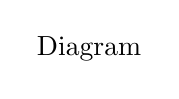
\begin{tikzpicture}
            \node {Diagram};
        \end{tikzpicture}
        \end{center}
    \item 
        \begin{tasks}(2)
            \task $I = \frac{V_0 t}{\pi \rho} \ln\left(\frac{R_2}{R_1}\right)$
            \task the outer surface is at a higher voltage than the inner surface
            \task the outer surface is at a lower voltage than the inner surface
            \task $\Delta V \propto I^2$
        \end{tasks}
\end{enumerate}
